\sect{Determinante}

\ssect{Definition}

Eine \textbf{$n$-reihige Determinante} ist eine reelle Zahl, die aus den Elementen einer reellen $n \times n$ Matrix nach bestimmten Vorschriften berechnet wird.

Für 2-reihige Determinanten: $\det(A) = \left|
\begin{array}{cc}
    a & b \\
    c & d \\
\end{array}
\right| = ad - cb$

Für 3-reihige Determinante: Regel von Sarrus

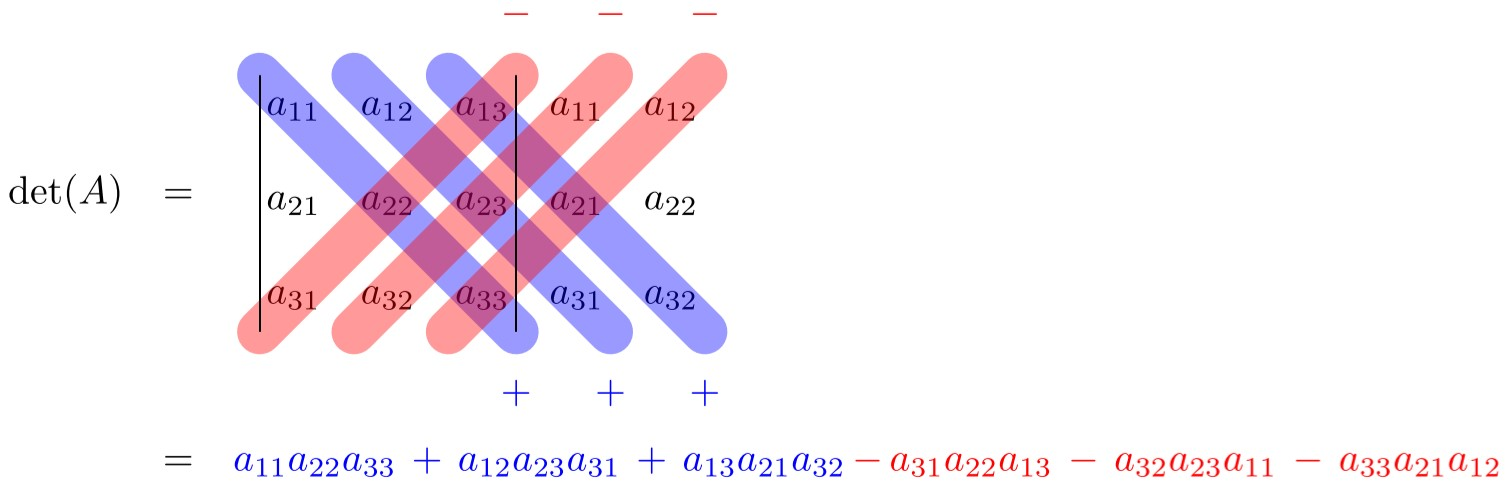
\includegraphics[scale=0.23]{regel-von-sarrus}

\ssect{Eigenschaften}

\textbf{Eigenschaft 1:} Die Matrix $A$ und ihre Transponierte $A^T$ besitzen dieselbe Determinante: $\det(A^T) = \det(A)$

\textbf{Eigenschaft 2:} Beim Vertauschen zweier Zeilen (oder Spalten) ändert eine Determinante ihr Vorzeichen.

\textbf{Eigenschaft 3:} Sei $A$ eine $n \times n$ Matrix.
Sei $\lambda$ eine reelle Zahl.
Dann gilt: $\det(\lambda A) = \lambda^n \det(A)$

\textbf{Eigenschaft 4:} Eine Determinante besitzt den Wert Null, wenn sie mind.\ eine der folgenden Bedingungen erfüllt:
\begin{enumerate}
    \item Alle Elemente einer Zeile (oder Spalte) sind Null.
    \item Zwei Zeilen (oder Spalten) stimmen überein.
    \item Eine Zeile (oder Spalte) ist als Linearkombination der übrigen Zeilen (oder Spalten) darstellbar.
\end{enumerate}

\textbf{Eigenschaft 5:} Der Wert einer Determinante ändert sich \textbf{nicht}, wenn man zu einer Zeile/Spalte ein beliebiges Vielfaches einer anderen Zeile/Spalte elementweise addiert.

\textbf{Eigenschaft 6:} Für zwei $n \times n$ Matrizen $A$ und $B$ gilt stets: \[\det(AB) = \det(A) \cdot \det(B)\]

\textbf{Eigenschaft 7:} Die Determinante einer Dreiecksmatrix ist gleich dem Produkt der Hauptdiagonalelemente.

\textbf{Eigenschaft 8:} Ist die Matrix invertierbar, dann gilt: \[\det(A^{-1}) = \frac{1}{\det(A)}\]

\ssect{Berechnung von n-reihigen Determinanten}

Sei $A$ eine $n \times n$ reelle Matrix.
Durch Weglassen der $i$-ten Zeile und der $j$-ten Spalte erhält man die $(n-1) \times (n-1)$  \textbf{Untermatrix} von $A$.
Ihre Determinante $\det(A_{ij})$ heisst die \textbf{Unterdeterminante von $A$}.

\textbf{Beispiel 1:} Die Untermatrix $A_{12}$ aus $A$ geht durch Streichen der 1.\ Zeile und 2.\ Spalte hervor:

Für $A = \left(
\begin{array}{c>{\columncolor{blue!40}}cc}
    \rowcolor{blue!40}
    a_{11} & a_{12} & a_{13} \\
    a_{21} & a_{22} & a_{23} \\
    a_{31} & a_{32} & a_{33}
\end{array}
\right)$ ist $A_{12} = \left(
\begin{array}{cc}
    a_{21} & a_{23} \\
    a_{31} & a_{33}
\end{array}
\right)$.

Die zugehörige Unterdeterminante ist:
\[\det(A_{12}) = \left|
\begin{array}{cc}
    a_{21} & a_{23} \\
    a_{31} & a_{33}
\end{array}
\right| = a_{21} a_{33} - a_{31} a_{23}\]

\textbf{Beispiel 2:}
{\fontsize{7.5}{0}
    \[\det(A_{11}) = \left|
    \begin{array}{>{\columncolor{blue!40}}ccc}
        \rowcolor{blue!40}
        a_{11} & a_{12} & a_{13} \\
        a_{21} & a_{22} & a_{23} \\
        a_{31} & a_{32} & a_{33}
    \end{array}
    \right| = \left|
    \begin{array}{cc}
        a_{22} & a_{23} \\
        a_{32} & a_{33}
    \end{array}
    \right| = a_{22} a_{33} - a_{32} a_{23}\]
    \[\det(A_{21}) = \left|
    \begin{array}{>{\columncolor{blue!40}}ccc}
        a_{11} & a_{12} & a_{13} \\
        \rowcolor{blue!40}
        a_{21} & a_{22} & a_{23} \\
        a_{31} & a_{32} & a_{33}
    \end{array}
    \right| = \left|
    \begin{array}{cc}
        a_{12} & a_{13} \\
        a_{32} & a_{33}
    \end{array}
    \right| = a_{12} a_{33} - a_{32} a_{13}\]
    \[\det(A_{31}) = \left|
    \begin{array}{>{\columncolor{blue!40}}ccc}
        a_{11} & a_{12} & a_{13} \\
        a_{21} & a_{22} & a_{23} \\
        \rowcolor{blue!40}
        a_{31} & a_{32} & a_{33}
    \end{array}
    \right| = \left|
    \begin{array}{cc}
        a_{12} & a_{13} \\
        a_{22} & a_{23}
    \end{array}
    \right| = a_{12} a_{23} - a_{22} a_{13}\]
}

Damit lässt sich die Determinante auch in der folgenden Form darstellen: \[\det(A) = a_{11} \det(A_{11}) - a_{21} \det(A_{21}) + a_{31} \det(A_{31})\]

\sssect{Laplacescher Entwicklungssatz}

Eine $n$-reihige Determinante lässt sich nach den Elementen einer beliebigen Zeile oder Spalte wie folgt entwickeln:

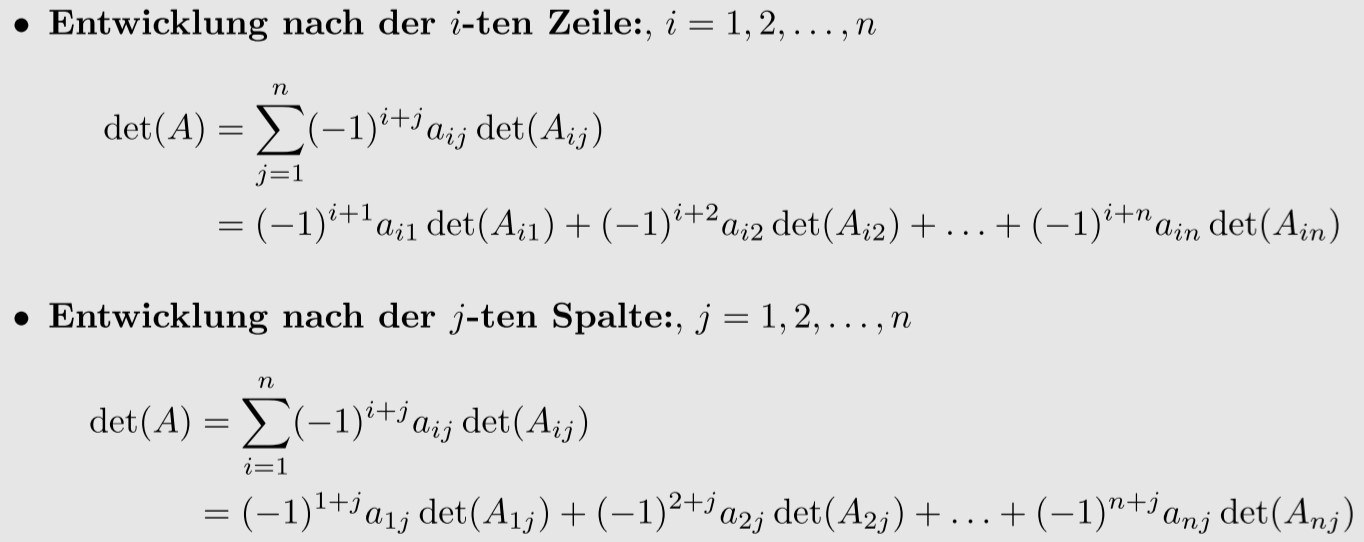
\includegraphics[scale=0.255]{laplacescher-entwicklungssatz}

\textbf{Anmerkung:}
\begin{itemize}
    \item Der Wert der Determinante ist \textbf{unabhängig} von der Entwicklungszeile oder -spalte.
    \item Es wird nach derjenigen Zeile/Spalte entwickelt, die die meisten Nullen enthält.
    \item Der Vorzeichenfaktor kann wiederum nach der Schachbrettregel bestimmt werden.
\end{itemize}
\vspace{-0.7em}
\begin{center}
    \begin{tabular}{|c|c|c|}
        \hline
        + & - & + \\
        \hline
        - & + & - \\
        \hline
        + & - & + \\
        \hline
    \end{tabular}
\end{center}
\vspace{-0.7em}

\ssect{Determinanten und LGS}

Die folgenden Aussagen sind äquivalent:
\begin{itemize}
    \item $\det(A) = 0$
    \item Der Rang von $A$ ist kleiner als $n$: $\text{rang}(A) < n$
    \item Das LGS $A \vec{x} = \vec{b}$ hat keine eindeutige Lösung.
    \item Die Matrix $A$ ist nicht invertierbar.
\end{itemize}

Die folgenden Aussagen sind ebenfalls äquivalent:
\begin{itemize}
    \item $\det(A) \neq 0$
    \item Der Rang von $A$ ist gleich $n$: $\text{rang}(A) = n$
    \item Das LGS $A \vec{x} = \vec{b}$ hat genau eine Lösung: $\vec{x} = A^{-1}\vec{b}$
    \item Die Matrix $A$ ist invertierbar.
\end{itemize}

\sssect{Geometrische Interpretation}

Der Betrag einer Determinante entspricht
\begin{itemize}
    \item dem \textbf{Flächeninhalt} einer $2 \times 2$ Matrix
    \item dem \textbf{Volumen} einer $3 \times 3$ Matrix
\end{itemize}
\[A = |\vec{a} \times \vec{b}| = \left| \det \left(
\begin{array}{cc}
    a_1 & b_1 \\
    a_2 & b_2
\end{array}
\right)\right|\]